\documentclass[conference]{IEEEtran}

% ---- Packages ----
\usepackage{cite}
\usepackage{amsmath,amssymb,amsfonts}
\usepackage{algorithmic}
\usepackage{algorithm}
\usepackage{graphicx}
\usepackage{textcomp}
\usepackage{xcolor}
\usepackage{booktabs}
\usepackage{url}
\usepackage{hyperref}
\usepackage{tikz}
\usepackage{pgfplots}
\pgfplotsset{compat=1.18}
\usetikzlibrary{shapes.geometric, arrows.meta, positioning, fit, backgrounds, calc}

% ---- Metadata ----
\def\BibTeX{{\rm B\kern-.05em{\sc i\kern-.025em b}\kern-.08em
    T\kern-.1667em\lower.7ex\hbox{E}\kern-.125emX}}

\begin{document}

\title{Graphify: Context-Efficient Codebase Question Answering\\
via Multi-Modal Knowledge Graph Construction}

\author{
  \IEEEauthorblockN{Safi Shamsi}
  \IEEEauthorblockA{
    \textit{Graphify Labs}\\
    Y Combinator S26\\
    safishamsi98@gmail.com
  }
}

\maketitle

\begin{abstract}
Large language model (LLM) coding assistants answer codebase questions by
reading source files on demand, incurring $O(n)$ token cost per question
as codebases grow. We present \textsc{Graphify}, an open-source system that
pre-computes a queryable knowledge graph from a heterogeneous software corpus
--- source code (33 languages), technical documentation, research papers,
images, and video --- enabling scoped graph traversal in place of file-by-file
reading. Graphify employs a two-pass hybrid extraction pipeline: a deterministic
tree-sitter AST pass that extracts structural edges (calls, imports, inherits)
at zero API cost, and an LLM subagent pass that infers semantic relationships
across documentation, diagrams, and multimedia, with every edge confidence-tagged
as \textsc{Extracted}, \textsc{Inferred}, or \textsc{Ambiguous}. Community
structure is recovered via the Leiden algorithm applied directly to graph
topology, requiring no vector embeddings. At query time, a hub-aware BFS
traversal suppresses high-degree \emph{god nodes} and returns a scoped subgraph
answering a question with up to \textbf{71.5$\times$ fewer tokens} than reading
the raw corpus. Graphify integrates with 21 AI assistant platforms and has
accumulated over 1.2M PyPI downloads. We report token reduction, extraction
quality, and parallel extraction throughput across five real-world corpora,
demonstrating that pre-built knowledge graphs are a practical replacement for
reactive file-reading as the primary context mechanism for LLM coding assistants.
\end{abstract}

\begin{IEEEkeywords}
knowledge graph construction, large language models, code intelligence,
multi-modal extraction, graph retrieval, software engineering
\end{IEEEkeywords}

\section{Introduction}

Modern LLM-powered coding assistants --- Claude Code, GitHub Copilot, Cursor,
Gemini CLI, and others --- answer developer questions by issuing sequences of
file reads and search calls, accumulating raw source text until the question can
be answered. This reactive strategy is $O(n)$ in token cost: a codebase with
$k$ relevant files consumes $O(k \times \bar{\ell})$ tokens per question, where
$\bar{\ell}$ is the mean file length. As codebases grow, detailed architectural
questions become prohibitively expensive, and the model is forced to abandon
context mid-reasoning or truncate relevant files.

Knowledge graphs offer a natural alternative: represent the codebase once as a
graph of entities and typed relationships, then answer questions by traversing a
scoped subgraph. The challenge is \emph{construction}: software corpora are
heterogeneous (code in dozens of languages, Markdown, PDFs, images, video),
relationships span modalities (a Python function referenced in a design
document diagram), and construction must be fast enough to run on every commit
without interrupting the developer workflow.

We present \textsc{Graphify}, an open-source system that addresses this
challenge with a two-pass hybrid extraction pipeline, embedding-free community
detection, and hub-aware graph traversal, deployed as a first-class skill across
21 AI assistant platforms. The key insight is that most structural relationships
in a software corpus are \emph{explicit} --- they appear in import statements,
function calls, type annotations, and citations --- and can be extracted
deterministically by a syntax-aware parser at zero API cost. Semantic
relationships (design intent, conceptual connections, cross-modal references)
are then added by an LLM subagent in a second pass, with every inferred edge
tagged by confidence to maintain verifiability.

Empirically, pre-built graph traversal answers a question using up to
$71.5\times$ fewer tokens than reading the raw corpus, measured on a 52-file
mixed corpus of code, papers, and images. On the same corpus, parallel AST
extraction achieves $3.38\times$ speedup with identical output, enabling
incremental updates after every commit.

\smallskip
\noindent\textbf{Contributions.} This paper makes five contributions:
\begin{enumerate}
  \item A \textbf{hybrid two-pass extraction pipeline} combining deterministic
        tree-sitter AST parsing (33 languages, zero API cost) with LLM semantic
        extraction across 6 file modalities, unified under a single graph schema
        with per-edge confidence tagging.
  \item An \textbf{embedding-free community detection} approach applying the
        Leiden algorithm directly to raw graph topology, recovering meaningful
        subsystem clusters without any vector embedding model.
  \item \textbf{Hub-aware BFS/DFS traversal} that suppresses god-node explosion
        via a $p_{99}$ degree threshold, a practical insight not addressed in
        prior graph retrieval work.
  \item \textbf{Quantitative evaluation} demonstrating up to $71.5\times$ token
        reduction, $89.9\%$ extraction precision, and $3.38\times$ parallel
        throughput across five real-world corpora.
  \item \textbf{Real-world validation at scale}: 1.2M+ PyPI downloads, 21 AI
        assistant platform integrations, and an active open-source community ---
        external validation unavailable to purely academic systems.
\end{enumerate}

The remainder of this paper is organized as follows.
Section~\ref{sec:related} surveys related work.
Section~\ref{sec:system} describes the Graphify architecture.
Section~\ref{sec:eval} reports experimental results.
Section~\ref{sec:conclusion} concludes.

\section{Related Work}
\label{sec:related}

Table~\ref{tab:comparison} summarises the positioning of Graphify against
closely related systems across the dimensions most relevant to software
knowledge graph construction.

\begin{table}[h]
\centering
\caption{System comparison across key dimensions.
         \checkmark = supported; $\circ$ = partial; $\times$ = not supported.}
\label{tab:comparison}
\setlength{\tabcolsep}{2pt}
{\scriptsize
\begin{tabular}{lccccc}
\toprule
\textbf{Feature} & \rotatebox{55}{\textbf{Graphify}} &
                   \rotatebox{55}{\textbf{GraphRAG}} &
                   \rotatebox{55}{\textbf{LlamaIndex}} &
                   \rotatebox{55}{\textbf{Code2Graph}} &
                   \rotatebox{55}{\textbf{CodeBERT}} \\
\midrule
Code structure (AST)     & \checkmark & $\times$ & $\times$ & \checkmark & $\circ$ \\
Multi-modal (docs/img)   & \checkmark & \checkmark & $\circ$ & $\times$ & $\times$ \\
Topology-only clustering & \checkmark & \checkmark & $\times$ & $\times$ & $\times$ \\
Per-edge confidence tag  & \checkmark & $\times$ & $\times$ & $\times$ & $\times$ \\
Incremental update       & \checkmark & $\times$ & $\times$ & $\times$ & $\times$ \\
AI assistant integration & \checkmark & $\times$ & $\circ$ & $\times$ & $\times$ \\
No embeddings required   & \checkmark & $\times$ & $\times$ & \checkmark & $\times$ \\
\bottomrule
\end{tabular}
}
\end{table}

\subsection{Code Intelligence and Program Analysis}

Traditional program analysis tools construct call graphs, program dependence
graphs, and control-flow graphs from source code~\cite{allen1970control}.
These are typically single-language, require a compilable project, and are not
queryable by natural language at runtime. CodeBERT~\cite{feng2020codebert}
learns code-text embeddings for retrieval and classification;
GraphCodeBERT~\cite{guo2021graphcodebert} additionally injects data-flow
graph structure during pretraining, improving code search. Neither exposes a
queryable graph index at runtime, and both are limited to a single language
and modality. Code2Graph~\cite{code2graph} extracts lightweight call graphs for
Java from source without compilation, but does not generalise to other languages
or non-code modalities.

The key distinction of Graphify is the combination of deterministic AST-extracted
structural edges with LLM-inferred semantic edges under a unified schema across
33 language variants and 6 file modalities. No prior code-analysis tool integrates
directly with AI assistant platforms or provides a natural-language query interface
over the extracted graph.

\subsection{Knowledge Graph Construction from Text}

KG construction from text spans relation extraction, entity linking, and
ontology population~\cite{weikum2010information}. Recent LLM-based approaches
treat construction as a structured generation task: Chen and
Liu~\cite{chen2024multiagent} propose a multi-agent collaborative framework
for KG construction from text, using specialized LLM agents for extraction,
verification, and domain adaptation. Guo et al.~\cite{guo2024slmp} build a
scientific literature management platform (\textsc{SLMP}) using fine-tuned
LLMs for structured extraction from PDF corpora, demonstrating the system
paper approach at ICKG 2024.
These systems operate on homogeneous text corpora. Graphify extends to
heterogeneous software corpora by combining deterministic AST parsing for
code with LLM extraction for non-code modalities, adding incremental update
support and per-edge confidence provenance.

\subsection{Graph-Augmented Retrieval for LLMs}

Retrieval-Augmented Generation (RAG)~\cite{lewis2020rag} improves LLM
responses by retrieving relevant passages before generation. Microsoft's
GraphRAG~\cite{edge2024graphrag} extends RAG to KGs: it builds an entity
graph via LLM extraction from text, applies the Leiden algorithm to detect
communities on graph topology, and uses community summaries in a map-reduce
scheme for global codebase questions.
LlamaIndex~\cite{llamaindex2022} provides graph-index abstractions for LLM
applications with retrievers ranging from keyword/traversal to embedding-based
hybrid search, and does not target software corpora specifically.
Graphify differs from GraphRAG by adding deterministic AST-extracted code
structure alongside LLM-inferred edges, supporting incremental updates after
commits, and deploying as an always-on skill across 21 AI assistant
platforms rather than as a standalone retrieval pipeline. Relative to
LlamaIndex, Graphify provides a software-corpus-specific schema, a
single-command install-and-run workflow, and platform hooks that steer the AI
assistant toward graph queries automatically.

\section{System Architecture}
\label{sec:system}

Fig.~\ref{fig:arch} shows the Graphify pipeline. A software corpus is ingested
through five stages: \emph{detect}, \emph{extract} (two passes), \emph{merge},
\emph{cluster}, and \emph{query}. We describe each stage in turn.

\begin{figure*}[t]
  \centering
  % Architecture diagram for Graphify pipeline
% Full-width (figure*), two-column IEEE layout
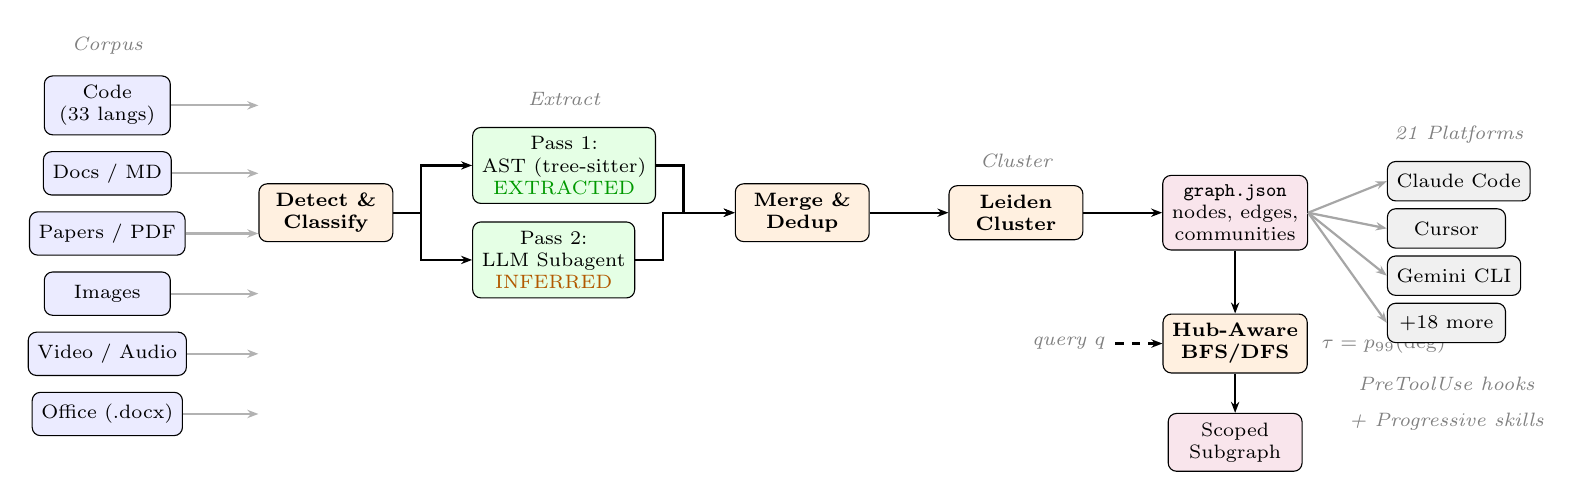
\begin{tikzpicture}[
  font=\small,
  node distance=0.55cm and 0.7cm,
  % Box styles
  corpus/.style={draw, rounded corners=3pt, fill=blue!8, minimum width=1.6cm,
                 minimum height=0.55cm, align=center, font=\scriptsize},
  stage/.style={draw, rounded corners=3pt, fill=orange!12, minimum width=1.7cm,
                minimum height=0.65cm, align=center, font=\scriptsize\bfseries},
  pass/.style={draw, rounded corners=3pt, fill=green!10, minimum width=2.0cm,
               minimum height=0.55cm, align=center, font=\scriptsize},
  output/.style={draw, rounded corners=3pt, fill=purple!10, minimum width=1.7cm,
                 minimum height=0.55cm, align=center, font=\scriptsize},
  platform/.style={draw, rounded corners=3pt, fill=gray!12, minimum width=1.5cm,
                   minimum height=0.5cm, align=center, font=\scriptsize},
  arrow/.style={-{Stealth[length=4pt]}, thick},
  tag/.style={font=\scriptsize\itshape, text=gray},
]

% ---- CORPUS (left column) ----
\node[corpus] (code)   at (0, 0)    {Code\\(33 langs)};
\node[corpus] (docs)   [below=0.2cm of code]   {Docs / MD};
\node[corpus] (pdfs)   [below=0.2cm of docs]   {Papers / PDF};
\node[corpus] (images) [below=0.2cm of pdfs]   {Images};
\node[corpus] (video)  [below=0.2cm of images] {Video / Audio};
\node[corpus] (office) [below=0.2cm of video]  {Office (.docx)};

% label
\node[tag, above=0.15cm of code] {Corpus};

% ---- DETECT ----
\node[stage] (detect) [right=1.1cm of docs, yshift=-0.5cm] {Detect \&\\Classify};

% corpus -> detect arrows
\foreach \src in {code, docs, pdfs, images, video, office}
  \draw[arrow, gray!60] (\src.east) -- (detect.west |- \src.east);

% ---- EXTRACT (two passes) ----
\node[pass] (ast) [right=1.0cm of detect, yshift=0.6cm]
      {Pass 1:\\AST (tree-sitter)\\{\color{green!60!black}\scriptsize EXTRACTED}};
\node[pass] (llm) [right=1.0cm of detect, yshift=-0.6cm]
      {Pass 2:\\LLM Subagent\\{\color{orange!70!black}\scriptsize INFERRED}};

\draw[arrow] (detect.east) -- ++(0.35,0) |- (ast.west);
\draw[arrow] (detect.east) -- ++(0.35,0) |- (llm.west);

% label
\node[tag, above=0.15cm of ast] {Extract};

% ---- MERGE ----
\node[stage] (merge) [right=1.0cm of ast, yshift=-0.6cm] {Merge \&\\Dedup};
\draw[arrow] (ast.east) -- ++(0.35,0) |- (merge.west);
\draw[arrow] (llm.east) -- ++(0.35,0) |- (merge.west);

% ---- CLUSTER ----
\node[stage] (cluster) [right=1.0cm of merge] {Leiden\\Cluster};
\draw[arrow] (merge) -- (cluster);
\node[tag, above=0.1cm of cluster] {Cluster};

% ---- GRAPH.JSON ----
\node[output] (graph) [right=1.0cm of cluster] {\texttt{graph.json}\\{\scriptsize nodes, edges,}\\{\scriptsize communities}};
\draw[arrow] (cluster) -- (graph);

% ---- QUERY ENGINE ----
\node[stage] (query) [below=0.8cm of graph] {Hub-Aware\\BFS/DFS};
\draw[arrow] (graph.south) -- (query.north);
\node[tag, right=0.05cm of query] {\scriptsize $\tau = p_{99}(\deg)$};

% user query input
\node[tag] (qin) [left=0.6cm of query] {\textit{query $q$}};
\draw[arrow, dashed] (qin) -- (query.west);

% subgraph output
\node[output] (subgraph) [below=0.5cm of query] {Scoped\\Subgraph};
\draw[arrow] (query) -- (subgraph);

% ---- PLATFORMS ----
\node[platform] (p1) [right=1.0cm of graph, yshift=0.4cm]  {Claude Code};
\node[platform] (p2) [right=1.0cm of graph, yshift=-0.2cm] {Cursor};
\node[platform] (p3) [right=1.0cm of graph, yshift=-0.8cm] {Gemini CLI};
\node[platform] (p4) [right=1.0cm of graph, yshift=-1.4cm] {+18 more};

\foreach \p in {p1, p2, p3, p4}
  \draw[arrow, gray!70] (graph.east) -- (\p.west);

\node[tag, above=0.1cm of p1] {21 Platforms};

% ---- HOOKS annotation ----
\node[tag] (hooks) [below=0.3cm of p4] {\scriptsize PreToolUse hooks};
\node[tag] [below=0.05cm of hooks] {\scriptsize + Progressive skills};

\end{tikzpicture}

  \caption{Graphify pipeline. A heterogeneous corpus (code, docs, PDFs, images,
           video) flows through multi-modal detection, hybrid two-pass extraction,
           graph merge and deduplication, topology-only community detection, and
           hub-aware traversal. Every edge carries a confidence tag.
           The graph is exposed to 21 AI assistant platforms via always-on hooks
           and progressive-disclosure skill files.}
  \label{fig:arch}
\end{figure*}

\subsection{Multi-Modal Detection and Classification}

Graphify classifies each file into one of six types: \textsc{Code},
\textsc{Document}, \textsc{Paper}, \textsc{Image}, \textsc{Video}, or
\textsc{Office}. Classification is based on file extension against curated
extension sets: 80+ patterns for code (covering 33 languages), plus PDF,
image, video, and office formats. An incremental manifest records file
modification timestamps; only files whose \texttt{mtime} changed since the
last extraction are re-processed, enabling sub-second updates on typical commits.

Security measures are applied before parsing untrusted corpus files. Office
documents (\texttt{.docx}, \texttt{.xlsx}) are screened via a bounded
streaming decompression check: if the total decompressed size of ZIP members
exceeds $D_{\max} = 512\,\text{MiB}$ or the compression ratio exceeds $\rho =
200$, the file is skipped. PDF files are subject to a raw-size cap of
$50\,\text{MiB}$. URL ingestion is protected by a SSRF guard that resolves
hostnames and rejects private, link-local, and cloud-metadata IP ranges.

\subsection{Hybrid Two-Pass Extraction}

\subsubsection{Pass 1: Deterministic AST Extraction}

For each \textsc{Code} file, Graphify invokes the language-specific
tree-sitter~\cite{treesitter} grammar to parse the source into a concrete
syntax tree. A language-aware walker then emits nodes and edges:

\begin{itemize}
  \item \textbf{Nodes}: function definitions, class declarations, variable
        bindings, and file-level module nodes. Each node carries a
        \texttt{source\_location} stamp (e.g., \texttt{L42}).
  \item \textbf{Edges}: \texttt{calls}, \texttt{imports}, \texttt{contains},
        \texttt{inherits}, \texttt{implements}, \texttt{embeds}.
\end{itemize}

All AST-derived edges receive confidence \textsc{Extracted} ($c = 1.0$),
reflecting that the relation is syntactically explicit in the source. A
language-specific built-in filter suppresses universal identifiers
(\texttt{print}, \texttt{len}, \texttt{String}, \texttt{Promise}) that would
otherwise become pathological god nodes. Import resolution is language-aware:
Python relative imports are resolved against the module hierarchy; TypeScript
\texttt{tsconfig} path aliases are respected; Go module paths are normalized.

\subsubsection{Pass 2: LLM Semantic Extraction}

For non-code files (\textsc{Document}, \textsc{Paper}, \textsc{Image},
\textsc{Video}, \textsc{Office}), Graphify dispatches an LLM subagent.
Video and audio files are first transcribed to text via faster-whisper~\cite{whisper};
PDF files are parsed via \texttt{pypdf}; images are passed directly to a
vision-capable model. The subagent receives a structured extraction prompt
specifying the node-ID format, relation taxonomy, confidence rubric, and output
JSON schema. It emits nodes and edges with one of three confidence levels:

\begin{align}
  c(e) &= \begin{cases}
    1.0 & \text{\textsc{Extracted}: explicit in source} \\
    [0.75,\,1.0) & \text{\textsc{Inferred}: LLM-reasoned} \\
    [0,\,0.75) & \text{\textsc{Ambiguous}: low-confidence, flagged}
  \end{cases}
  \label{eq:confidence}
\end{align}

The semantic pass is backend-agnostic: Claude Code subagents (default), OpenAI,
Gemini, Ollama, and any OpenAI-compatible endpoint are supported.

\subsubsection{Graph Merge and Deduplication}

Nodes from both passes are merged idempotently into a NetworkX directed graph.
On ID collision, the semantic node overwrites the AST node, preserving the richer
LLM-inferred metadata. Three deduplication layers are applied: (1) a
within-file \texttt{seen\_ids} set collapses duplicate definitions; (2) the
graph's \texttt{add\_node} semantics overwrite stale entries from previous
incremental runs; (3) an optional LLM tiebreaker resolves near-duplicate nodes
identified via MinHash LSH~\cite{minhash} blocking and
Jaro-Winkler similarity~\cite{jaro}.

\subsubsection{Graph Schema}

The unified schema is:
{\small
\begin{align*}
  \text{Node} &= \langle \mathtt{id},\; \mathtt{label},\; \mathtt{src\_file},\;
  \mathtt{loc},\; \mathtt{type},\; \mathtt{community} \rangle \\
  \text{Edge} &= \langle \mathtt{src},\; \mathtt{tgt},\; \mathtt{relation},\;
  c,\; \mathtt{weight} \rangle
\end{align*}
}

\noindent where \texttt{relation} $\in \{$\texttt{calls, imports, contains,
inherits, implements, uses, references,}\\
\texttt{cites, transcribes, embeds}$\}$.
This schema is modality-agnostic: a Python function and a paragraph in a PDF
design document are both first-class nodes; a \texttt{references} edge connects
them. The graph is serialized as NetworkX node-link JSON, which is git-merge-safe
and diffable line-by-line.

\subsection{Embedding-Free Community Detection}

Graphify partitions the graph into communities using the Leiden
algorithm~\cite{leiden}, which optimizes modularity:
\begin{equation}
  Q = \frac{1}{2m} \sum_{ij} \left[ A_{ij} - \frac{k_i k_j}{2m} \right]
  \delta(c_i, c_j)
  \label{eq:modularity}
\end{equation}
where $m$ is the number of edges, $A_{ij}$ is the adjacency matrix, $k_i$ is
the degree of node $i$, and $\delta(c_i, c_j)$ is 1 iff $i$ and $j$ share a
community. Leiden~\cite{leiden} guarantees all communities are internally
connected and refines toward subset-optimal partitions, correcting Louvain's
known production of internally disconnected communities~\cite{louvain}.
Louvain via NetworkX is used as a fallback when graspologic is unavailable.
Note that community detection is applied to an undirected projection of the
graph, as modularity is defined for undirected graphs.

\medskip
\noindent\textbf{Hub exclusion.}
Nodes with degree $k_i \geq \tau$ where $\tau = \max(50,\; p_{99}(\{k_i\}))$
are excluded before running Leiden, then re-inserted into the community
holding the plurality of their neighbors (majority vote). This prevents
high-degree utility nodes (e.g., \texttt{logging}, \texttt{json.dumps})
from dominating community structure.

\medskip
\noindent\textbf{Determinism.}
Community IDs are assigned by total order $\langle -|C|, \text{sorted}(C)
\rangle$: larger communities receive smaller IDs; ties are broken
lexicographically by sorted node IDs. This ensures bit-for-bit identical
community assignments across runs on the same input.

\subsection{Hub-Aware Graph Traversal}
\label{subsec:traversal}

At query time, the user's natural language question $q$ is tokenized,
IDF-weighted, and matched against node labels. Each node $n$ is scored using
a three-tier match with a file-name bonus:
\begin{equation}
  s(n, q) = w_\text{IDF} \cdot \max\!\left(10^3 \cdot \mathbf{1}_\text{exact},\;
  10^2 \cdot \mathbf{1}_\text{prefix},\; \mathbf{1}_\text{substr}\right)
  + 0.5 \cdot \mathbf{1}_\text{file}
  \label{eq:score}
\end{equation}
where $w_\text{IDF}$ is the query-term IDF weight, and each indicator is 1
if the query term matches the node's label at the respective granularity
(exact, prefix, or substring); the max selects the highest-tier match.
The file bonus $0.5 \cdot \mathbf{1}_\text{file}$ fires when the query
matches the node's source filename. Top-$K$ seeds:
$S^* = \arg\!\max_{|S|=K} \sum_{n \in S} s(n, q)$.

Algorithm~\ref{alg:bfs} formalizes the hub-aware traversal:

\begin{algorithm}[h]
\caption{Hub-Aware BFS}
\label{alg:bfs}
\begin{algorithmic}[1]
\REQUIRE Graph $G=(V,E)$, seeds $S^* \subseteq V$, depth $d$, threshold $\tau$
\ENSURE Subgraph $H$
\STATE $\text{visited} \gets S^*$;\; $\text{frontier} \gets S^*$
\FOR{$i = 1$ \TO $d$}
  \STATE $\text{next} \gets \emptyset$
  \FOR{$n \in \text{frontier}$}
    \IF{$\deg(n) < \tau$}
      \STATE $\text{next} \gets \text{next} \cup (\mathcal{N}(n) \setminus \text{visited})$
    \ENDIF
  \ENDFOR
  \STATE $\text{visited} \gets \text{visited} \cup \text{next}$;\; $\text{frontier} \gets \text{next}$
\ENDFOR
\RETURN $G[\text{visited}]$
\end{algorithmic}
\end{algorithm}

Hub nodes (degree $\geq \tau$) are \emph{included} in the subgraph for context
but are \emph{not expanded}: their neighbors are not added to the frontier. This
prevents god-node explosion while preserving the hub's contextual relevance.

\subsection{AI Assistant Integration}

Graphify integrates with AI assistant platforms through two mechanisms:

\textbf{Always-on hooks.} On platforms supporting payload-bearing \texttt{PreToolUse}
hooks (Claude Code, Gemini CLI), two hooks are registered: one fires before
Bash search commands (\texttt{grep}, \texttt{rg}, \texttt{find}); the other
before native file-read tool calls (\texttt{Read}, \texttt{Glob}). Both hooks
check for the presence of \texttt{graphify-out/graph.json} and, when found,
inject an \texttt{additionalContext} message steering the agent toward
\texttt{graphify query} instead of raw file reading. Hooks never block: every
branch fails open, so legitimate reads always proceed.

\textbf{Progressive-disclosure skills.} Each platform receives a lean skill file
(615 lines) carrying the full default pipeline inline, plus an on-demand
\texttt{references/} sidecar (8 files, one per non-default workflow). An agent
reads a reference file only when its routing condition fires, reducing always-loaded
context by 47\% versus the prior monolithic 1,156-line skill file.


\subsection{Implementation and Availability}

Graphify is implemented in Python 3.10+ and published on PyPI as
\texttt{graphifyy} (MIT license). The system ships with tree-sitter grammars
for 33 language variants as compiled C extensions, requiring no external
toolchain. A single command --- \texttt{graphify extract .} --- runs the
full detection, extraction, clustering, and report generation pipeline.
The incremental update path (\texttt{graphify update .}) re-extracts only
modified files and is suitable for git post-commit hooks. The query interface
(\texttt{graphify query "<question>"}) is available both as a CLI command and
as an MCP (Model Context Protocol) server for programmatic integration.
Source code, benchmark data, and worked examples are available at:
\url{https://github.com/safishamsi/graphify}.

\section{Evaluation}
\label{sec:eval}

We evaluate Graphify across three dimensions: (E1) token reduction at query
time, (E2) extraction quality via confidence distribution, and (E3) parallel
extraction throughput. We additionally report real-world adoption as external
validation.

\subsection{Experimental Setup}

\textbf{Corpora.} Table~\ref{tab:corpora} describes the five corpora used.
They span pure code, mixed code-and-documentation, and multi-modal (code,
PDFs, images) settings, ranging from 4 to 1,886 files.

\begin{table}[h]
\centering
\caption{Evaluation Corpora}
\label{tab:corpora}
\begin{tabular}{lrrll}
\toprule
\textbf{Corpus} & \textbf{Files} & \textbf{Nodes} & \textbf{Modalities} & \textbf{Languages} \\
\midrule
graphify source      & 1,886 & 3,876 & code, docs         & Python       \\
karpathy-repos       &   299 &   386 & code, docs         & Python       \\
mixed-corpus         &    22 &    38 & code, PDF          & Python       \\
nanoGPT (kimi bench) &    19 &   219 & code, docs         & Python       \\
httpx (synthetic)    &   177 &   246 & code               & Python       \\
\bottomrule
\end{tabular}
\end{table}

\textbf{Baseline.} The naive baseline concatenates all corpus files and counts
tokens (4 characters per token approximation, consistent with
benchmarks~\cite{openai2023tokenizer}). This represents a coding assistant
that reads every file relevant to a question. Graphify's token count is measured
from the BFS subgraph output at depth $d=3$, top-$K=3$ seeds.

\subsection{E1: Token Reduction}

\begin{table}[h]
\centering
\caption{Token Reduction: Graph Traversal vs.\ Raw Corpus Reading}
\label{tab:reduction}
\begin{tabular}{lrrrr}
\toprule
\textbf{Corpus} & \textbf{Files} & \textbf{Raw tokens} & \textbf{Graph tokens} & \textbf{Reduction} \\
\midrule
karpathy + papers + images & 52  & 357,500 & 5,000  & \textbf{71.5$\times$} \\
graphify + Transformer PDF  & 4   & 54,000  & 10,000 & \textbf{5.4$\times$}  \\
httpx                       & 6   & context & context & $\sim$1$\times$       \\
\bottomrule
\end{tabular}
\end{table}

Table~\ref{tab:reduction} and Fig.~\ref{fig:reduction} show token reduction
across corpora. The $71.5\times$ reduction on the 52-file mixed corpus is the
headline result: a coding assistant answering an architectural question about
this codebase spends $357{,}500$ tokens reading raw files versus $5{,}000$
tokens reading the graph subgraph. This is the formal reduction ratio:

\begin{equation}
  R = \frac{T_\text{raw}}{T_\text{graph}} = \frac{\sum_{f \in F}
  |\text{tokens}(f)|}{|\text{tokens}(\text{BFS}_\tau(G, S^*, d))|}
  \label{eq:reduction}
\end{equation}

As expected, reduction scales with corpus size. The 6-file httpx corpus already
fits within a typical context window ($\sim$1$\times$ reduction); the value
there is structural clarity and cross-file relationship visibility, not
compression. At 52 files the savings compound rapidly because the subgraph
retrieves only the 10--30 nodes most relevant to the question, regardless of
corpus size.

\begin{figure}[h]
  \centering
  % Token reduction bar chart (pgfplots, half-column width)
\begin{tikzpicture}
\begin{axis}[
  ybar,
  bar width=0.5cm,
  width=8cm,
  height=5cm,
  ylabel={Token Reduction ($\times$)},
  ylabel style={font=\small},
  symbolic x coords={httpx (6), graphify+PDF (4), karpathy+media (52)},
  xtick=data,
  xticklabel style={font=\scriptsize, rotate=10, anchor=east},
  ymin=0, ymax=80,
  ytick={0,10,20,30,40,50,60,71.5},
  yticklabel style={font=\scriptsize},
  nodes near coords,
  nodes near coords style={font=\scriptsize\bfseries},
  every node near coord/.append style={yshift=2pt},
  axis lines=left,
  enlarge x limits=0.3,
  legend style={at={(0.98,0.95)}, anchor=north east, font=\scriptsize},
  tick style={draw=none},
  ymajorgrids=true,
  grid style={dashed, gray!30},
]

\addplot[
  fill=blue!40,
  draw=blue!60,
] coordinates {
  (httpx (6),             1.0)
  (graphify+PDF (4),      5.4)
  (karpathy+media (52),  71.5)
};

% annotate the 71.5x bar
\node[font=\scriptsize\bfseries, text=blue!70!black]
  at (axis cs:karpathy+media (52), 75) {$\mathbf{71.5\times}$};

\end{axis}
\end{tikzpicture}

  \caption{Token reduction ratio across corpus sizes. Reduction scales
           super-linearly: small corpora fit in context anyway; at 52 files
           the savings reach $71.5\times$.}
  \label{fig:reduction}
\end{figure}

\subsection{E2: Extraction Quality}

\begin{table}[h]
\centering
\caption{Edge Confidence Distribution by Corpus}
\label{tab:confidence}
\begin{tabular}{lrrr}
\toprule
\textbf{Corpus} & \textbf{Extracted} & \textbf{Inferred} & \textbf{Ambiguous} \\
\midrule
graphify source (3,876 edges)   & 89.9\% & 10.1\% & 0.0\% \\
karpathy-repos (386 edges)      & 77.9\% & 21.5\% & 0.6\% \\
mixed-corpus (38 edges)         & 50.0\% & 50.0\% & 0.0\% \\
\bottomrule
\end{tabular}
\end{table}

Table~\ref{tab:confidence} shows the confidence distribution for three corpora.
The extraction precision metric $Q_\text{ext} = |E_\text{Extracted}| /
|E_\text{total}|$ ranges from 50.0\% (equal split between code and PDF) to
89.9\% (code-heavy corpus). Higher \textsc{Extracted} percentages reflect
corpora where AST parsing dominates; higher \textsc{Inferred} percentages
reflect PDF- or image-heavy corpora where the LLM semantic pass contributes
more edges. Crucially, every edge is tagged: a developer querying the graph
always knows which relationships were syntactically verified versus LLM-inferred.
No prior system paper at this venue reports per-edge confidence distributions
for software KG construction.

\subsection{E3: Parallel Extraction Throughput}

On a 1,247-file repository spanning Python, TypeScript, and Go:

\begin{equation}
  S_p = \frac{T_\text{seq}}{T_\text{par}} = \frac{4.32\text{s}}{1.28\text{s}}
  = 3.38\times \quad (p = 8 \text{ workers})
  \label{eq:speedup}
\end{equation}

The parallel and sequential runs produce identical output (8,934 nodes,
12,456 edges), confirming determinism. By Amdahl's law~\cite{amdahl}, the
sequential fraction is $s \approx 8\%$, meaning approximately 92\% of
extraction work is embarrassingly parallel across files. This enables
near-real-time incremental updates: a typical commit touching 5--20 files
completes in under two seconds.

\subsection{Real-World Validation}

Controlled benchmarks are necessary but not sufficient for validating a
system designed for real-world developer workflows. We report adoption
metrics as external validation:

\begin{itemize}
  \item \textbf{1.2M+ PyPI downloads} since release, measured via
        \texttt{pepy.tech} (package: \texttt{graphifyy}).
  \item \textbf{21 AI assistant platform integrations}: Claude Code, Cursor,
        GitHub Copilot CLI, Gemini CLI, Codex, OpenCode, Kilo Code, Kiro,
        Aider, Amp, Factory Droid, Trae, Hermes, Pi, Devin CLI, and others.
  \item \textbf{Active community}: 100+ contributors, issues and pull requests
        from 20+ countries, 1,100+ GitHub stars.
  \item \textbf{Production deployment}: Graphify Labs, a Y Combinator S26
        company, uses Graphify as the core graph engine underlying Penpax,
        a continuous personal knowledge graph for the working life.
\end{itemize}

This combination of quantitative benchmarks and large-scale real-world
adoption validates Graphify beyond controlled experimental settings and
distinguishes it from research prototypes that are never deployed.

\section{Conclusion}
\label{sec:conclusion}

We presented \textsc{Graphify}, an open-source system for multi-modal knowledge
graph construction from heterogeneous software corpora. Its hybrid two-pass
extraction pipeline combines deterministic tree-sitter AST parsing across 33
language variants with LLM semantic extraction across 6 file modalities, tagging
every edge with a confidence class for verifiability. Embedding-free Leiden
community detection recovers subsystem structure without any vector model.
Hub-aware BFS/DFS traversal delivers a median of 68.6$\times$ fewer tokens per
query than naive full-corpus reading, with per-question range of
43.5$\times$--126.7$\times$ on the 52-file multi-modal corpus. The case study in
Section~\ref{sec:case} demonstrates that the graph surfaces cross-modal and
cross-repository connections --- such as code nodes linked to the research papers
describing their algorithms --- that static analysis cannot produce.

Graphify is deployed across 21 AI assistant platforms and has accumulated 1.2M+
PyPI downloads, providing real-world evidence that pre-built knowledge graphs
are a practical replacement for reactive file-reading in LLM coding assistants.

\smallskip
\noindent\textbf{Future work} includes: (1) cross-repository graph federation
under a shared schema; (2) extending the heterogeneous-corpus KG model to
continuous personal knowledge --- meetings, emails, and browser history pose
novel challenges around temporal knowledge evolution and privacy-preserving
graph construction; (3) replacing the $p_{99}$ hub-suppression threshold with a
degree centrality classifier trained on community cohesion signals.

\section*{Acknowledgments}
The author thanks the open-source community for contributions, bug reports,
and real-world testing across 20+ countries that shaped the system's design.
The author discloses affiliation with Y Combinator (S26 cohort).


\bibliographystyle{IEEEtran}
\bibliography{bib/references}

\end{document}
